%----------------------------------------------------------------------------------------
%	PACKAGES AND OTHER DOCUMENT CONFIGURATIONS
%----------------------------------------------------------------------------------------

\documentclass[
12pt, % The default document font size, options: 10pt, 11pt, 12pt
%oneside, % Two side (alternating margins) for binding by default, uncomment to switch to one side
english, % ngerman for German
onehalfspacing, % Single line spacing, alternatives: onehalfspacing or doublespacing
%draft, % Uncomment to enable draft mode (no pictures, no links, overfull hboxes indicated)
%nolistspacing, % If the document is onehalfspacing or doublespacing, uncomment this to set spacing in lists to single
%liststotoc, % Uncomment to add the list of figures/tables/etc to the table of contents
%toctotoc, % Uncomment to add the main table of contents to the table of contents
%parskip, % Uncomment to add space between paragraphs
%nohyperref, % Uncomment to not load the hyperref package
headsepline, % Uncomment to get a line under the header
%chapterinoneline, % Uncomment to place the chapter title next to the number on one line
%consistentlayout, % Uncomment to change the layout of the declaration, abstract and acknowledgements pages to match the default layout
]{MastersDoctoralThesis} % The class file specifying the document structure


\usepackage[utf8]{inputenc} % Required for inputting international characters
\usepackage[T1]{fontenc} % Output font encoding for international characters
\usepackage{tabularx}
\usepackage{mathpazo} % Use the Palatino font by default
\usepackage{amssymb}
\usepackage{pifont}
\usepackage{booktabs}
\usepackage{changepage}
\usepackage{csquotes}
\usepackage{bm}
\usepackage{adjustbox}
\usepackage{tabularx}
\usepackage{tabulary}
\usepackage{graphicx}% Include figure files
\usepackage{dcolumn}% Align table columns on decimal point
\usepackage{tabularray}


\usepackage[style=authoryear-icomp,maxbibnames=9,maxcitenames=2,backend=biber]{biblatex}


% \usepackage[autostyle=true]{csquotes} % Required to generate language-dependent quotes in the bibliography

\addbibresource{bibliography.bib}

\usepackage{graphicx}
\usepackage{xurl}
\usepackage{hyperref}
\usepackage{pifont}
\usepackage{amssymb}
\usepackage{xcolor,colortbl}
\usepackage{microtype}
\setlength{\emergencystretch}{2em} % fewer overfull lines from long hyphenated model names
\makeatletter
\newcommand{\tabinput}[1]{\@@input #1 } % primitive \input, safe inside tabulars before \bottomrule
\makeatother
\newcommand{\cmark}{\ding{51}}%
\newcommand{\xmark}{\ding{55}}%
%----------------------------------------------------------------------------------------
%	MARGIN SETTINGS
%----------------------------------------------------------------------------------------

\geometry{
	paper=a4paper, % Change to letterpaper for US letter
	inner=2.5cm, % Inner margin
	outer=2.5cm, % Outer margin
	bindingoffset=.5cm, % Binding offset
	top=2cm, % Top margin
	bottom=2cm, % Bottom margin
	%showframe, % Uncomment to show how the type block is set on the page
}

%----------------------------------------------------------------------------------------
%	THESIS INFORMATION
%----------------------------------------------------------------------------------------

\thesistitle{Plain Language Summarization of Clinical Trials}
\supervisor{Dr. Grigorios \textsc{Tsoumakas}}
\degree{Master of Science}
\author{Grigorios \textsc{Barmpas}}
\university{Aristotle University of Thessaloniki}
\department{Department of Computer Science}
\faculty{Faculty Name}

% \AtBeginDocument{
%     \hypersetup{pdftitle=\ttitle} % Set the PDF's title to your title
%     \hypersetup{pdfauthor=\authorname} % Set the PDF's author to your name
%     \hypersetup{pdfkeywords=\keywordnames} % Set the PDF's keywords to your keywords
% }

\begin{document}
\selectlanguage{english}
\frontmatter % Use roman page numbering style (i, ii, iii, iv...) for the pre-content pages

\pagestyle{plain} % Default to the plain heading style until the thesis style is called for the body content

\hyphenation{Tsou-ma-kas Blo-om-berg}

%----------------------------------------------------------------------------------------
%	TITLE PAGE
%----------------------------------------------------------------------------------------

\begin{titlepage}
\begin{center}

\vspace*{.06\textheight}
{\scshape\LARGE \univname\par}\vspace{1.5cm}
\textsc{\Large Master's Thesis}\\[0.5cm]

\HRule \\[0.4cm] % Horizontal line
{\huge \ttitle\par}\vspace{0.4cm}
\HRule \\[1.5cm] % Horizontal line
 
\begin{minipage}[t]{0.4\textwidth}
\begin{flushleft} \large
\emph{Author:}\\
\authorname
\end{flushleft}
\end{minipage}
\begin{minipage}[t]{0.4\textwidth}
\begin{flushright} \large
\emph{Supervisor:} \\
\supname  
\end{flushright}
\end{minipage}\\[3cm]
 
\vspace{-3em}
\large \textit{A thesis submitted in fulfillment of the requirements\\ for the degree of \degreename}\\[0.3cm]
\textit{in the}\\[0.4cm]
\deptname\\[2cm]
\vspace{-3em}
\begin{center}
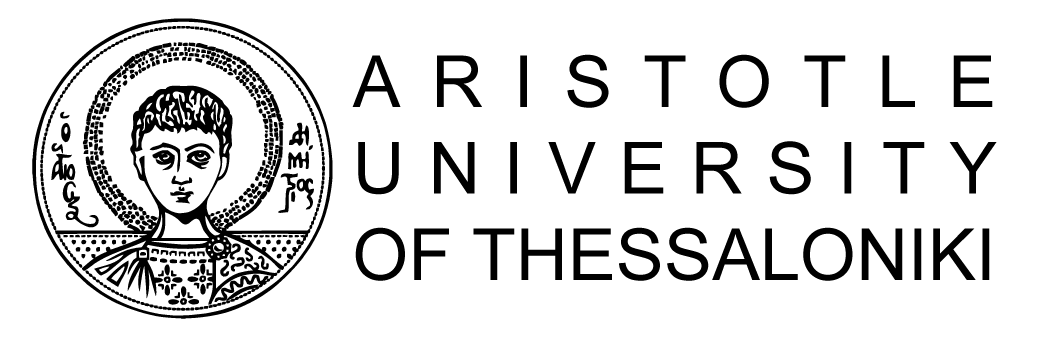
\includegraphics[width=4cm, trim={0cm 0.8cm 0cm 0.6cm}, clip]{Figures/logo.png}     
\end{center}
% \vspace{-2em}
\vfill
% \includegraphics[width=4cm]{Logo} % University/department logo - uncomment to place it
{\large \today}\\[4cm] % Date

 
\vfill
\end{center}
\end{titlepage}

%----------------------------------------------------------------------------------------
%	ABSTRACT PAGE
%----------------------------------------------------------------------------------------

\begin{abstract}
\addchaptertocentry{Abstract}
Clinical trial results are reported in technical language that patients and the public cannot easily use, and EU regulation now requires sponsors to publish summaries understandable to laypersons. This thesis studies the automatic generation of such plain-language summaries. From 561 Novartis clinical-trial PDFs we build a dataset of 959 examples from 212 usable trials, each pairing a patient question and the mapped section of the technical results report with the corresponding answer from the trial's patient summary, split by trial into training, validation and test sets. On a held-out test set of 138 examples from 31 trials we compare extractive baselines, an extractive question-answering model, zero-shot instruction-tuned models and fine-tuned Flan-T5 models, all trained and run on a CPU, with trial-level bootstrap confidence intervals and Holm-corrected paired tests. Fine-tuned Flan-T5-small reaches a ROUGE-L of 22.36 $\pm$ 0.39 over three seeds, roughly double the Lead-3 baseline (11.41), and matches the length and readability of human patient summaries. The evaluation, however, is fragile. No reference occurs verbatim in its source, so the extractive framing of earlier work cannot model the task. Decoding settings alone change the conclusions: under plain greedy decoding, ROUGE ranks a model that loops in 86\% of its outputs above Lead-3. Qualitative inspection and string-level faithfulness proxies suggest that the automatic metrics reward the style of patient summaries more than their correctness, and that the dataset construction encourages unsupported details, since the references contain many numbers absent from the model input. A human evaluation, prepared but not yet carried out, is needed to confirm this.
\end{abstract}

% Dedication
\cleardoublepage\thispagestyle{empty} 
\vspace*{5cm} 
\begin{center} 
....To my family....
\end{center}
\vfill 
     

%----------------------------------------------------------------------------------------
%	ACKNOWLEDGEMENTS
%----------------------------------------------------------------------------------------

\begin{acknowledgements}
\addchaptertocentry{\acknowledgementname} % Add the acknowledgements to the table of contents
I would like to sincerely thank my supervisor, Dr. Grigorios Tsoumakas, for his guidance and support throughout this thesis. His knowledge and encouragement have been a great help along the way.

I am also grateful to the professors of the master’s program for their teachings, which have played an important role in my academic growth.

Finally, I would like to thank my friends and family for their constant support and motivation throughout this journey.

\end{acknowledgements}

\selectlanguage{greek}
\chapter{Περίληψη στα Ελληνικά}
\addchaptertocentry{Περίληψη στα Ελληνικά}
Τα αποτελέσματα των κλινικών δοκιμών δημοσιεύονται σε τεχνική γλώσσα, την οποία οι ασθενείς και το ευρύ κοινό δύσκολα αξιοποιούν, ενώ ο ευρωπαϊκός κανονισμός απαιτεί πλέον από τους χορηγούς να δημοσιεύουν περιλήψεις κατανοητές από μη ειδικούς. Η εργασία μελετά την αυτόματη παραγωγή τέτοιων περιλήψεων σε απλή γλώσσα. Από 561 αρχεία \foreignlanguage{english}{PDF} κλινικών δοκιμών της \foreignlanguage{english}{Novartis} κατασκευάζεται σύνολο δεδομένων 959 παραδειγμάτων από 212 αξιοποιήσιμες δοκιμές. Κάθε παράδειγμα συνδέει μια ερώτηση ασθενούς και την αντίστοιχη ενότητα της τεχνικής αναφοράς αποτελεσμάτων με την απάντηση της περίληψης για ασθενείς, και ο διαχωρισμός σε σύνολα εκπαίδευσης, επικύρωσης και ελέγχου γίνεται ανά δοκιμή. Σε σύνολο ελέγχου 138 παραδειγμάτων από 31 δοκιμές συγκρίνονται εξαγωγικές μέθοδοι αναφοράς, ένα μοντέλο εξαγωγικής απάντησης ερωτήσεων, μοντέλα οδηγιών χωρίς εκπαίδευση στην εργασία και μοντέλα \foreignlanguage{english}{Flan-T5} με προσαρμογή (\foreignlanguage{english}{fine-tuning}), όλα σε υπολογιστή χωρίς κάρτα γραφικών, με διαστήματα εμπιστοσύνης \foreignlanguage{english}{bootstrap} σε επίπεδο δοκιμής και ζευγαρωτούς ελέγχους με διόρθωση \foreignlanguage{english}{Holm}. Το προσαρμοσμένο \foreignlanguage{english}{Flan-T5-small} πετυχαίνει \foreignlanguage{english}{ROUGE-L} 22.36 $\pm$ 0.39 σε τρεις σπόρους, περίπου διπλάσιο από τη μέθοδο αναφοράς \foreignlanguage{english}{Lead-3} (11.41), και πλησιάζει το μήκος και την αναγνωσιμότητα των ανθρώπινων περιλήψεων. Η αξιολόγηση όμως είναι εύθραυστη. Καμία περίληψη αναφοράς δεν εμφανίζεται αυτούσια στο κείμενο πηγής, άρα η εξαγωγική προσέγγιση προηγούμενης εργασίας δεν μπορεί να μοντελοποιήσει το πρόβλημα. Οι ρυθμίσεις αποκωδικοποίησης αρκούν για να αλλάξουν τα συμπεράσματα: με απλή άπληστη αποκωδικοποίηση, το \foreignlanguage{english}{ROUGE} κατατάσσει πάνω από το \foreignlanguage{english}{Lead-3} ένα μοντέλο που επαναλαμβάνεται κυκλικά στο 86\% των εξόδων του. Η ποιοτική εξέταση και δείκτες πιστότητας σε επίπεδο συμβολοσειρών υποδεικνύουν ότι οι αυτόματες μετρικές ανταμείβουν περισσότερο το ύφος των περιλήψεων για ασθενείς παρά την ορθότητά τους, και ότι ο τρόπος κατασκευής του συνόλου δεδομένων ευνοεί λεπτομέρειες χωρίς τεκμηρίωση, αφού οι περιλήψεις αναφοράς περιέχουν πολλούς αριθμούς που λείπουν από την είσοδο του μοντέλου. Για την επιβεβαίωση απαιτείται ανθρώπινη αξιολόγηση, η οποία έχει σχεδιαστεί αλλά δεν έχει ακόμη πραγματοποιηθεί.


\selectlanguage{english}

%----------------------------------------------------------------------------------------
%	LIST OF CONTENTS/FIGURES/TABLES PAGES
%----------------------------------------------------------------------------------------
\hypersetup{hidelinks}
\tableofcontents % Prints the main table of contents


\sloppy
\listoffigures % Prints the list of figures
 
\listoftables % Prints the list of tables
\fussy
%----------------------------------------------------------------------------------------
%	THESIS CONTENT - CHAPTERS
%----------------------------------------------------------------------------------------

\mainmatter % Begin numeric (1,2,3...) page numbering

\pagestyle{thesis} % Return the page headers back to the "thesis" style

% Include the chapters of the thesis as separate files from the Chapters folder
% Uncomment the lines as you write the chapters

% Chapter 1

\chapter{Introduction} % Main chapter title
\label{Chapter1}

\section{Problem Statement}

Clinical trial results are reported for specialists. A typical results report states objectives as statistical hypotheses, describes populations through inclusion and exclusion criteria, and reports outcomes as endpoints, hazard ratios and adverse-event tables. Patients, carers and most members of the public cannot use that text directly. Regulators have recognised the gap: in the European Union, Regulation (EU) No 536/2014 requires the sponsor of a clinical trial to provide, together with the summary of results, a summary written in a manner that is understandable to laypersons, with its content set out in Annex V of the Regulation \parencite[Art.~37(4)]{eu2014ctr}.

Writing these plain-language summaries (PLS) by hand is slow and requires both medical and communication expertise. This motivates automatic generation. The difficulty is that a useful PLS must do two things at once: change the register of the text (shorter sentences, everyday words, explained terms) and stay faithful to the trial. A fluent summary that states an outcome the trial did not report is worse than no summary.

This thesis revisits the plain-language summarisation study of the original MSc project \parencite{barmpas2024pls} with a rebuilt dataset, a corrected evaluation protocol and a broader set of systems. All experiments run on a CPU-only machine.

\section{Research Questions}

The study answers four research questions.

\begin{description}
    \item[RQ1.] Can small, CPU-trainable models generate plain-language answers that match human patient summaries better than extractive and zero-shot baselines?
    \item[RQ2.] Does the extractive question-answering framing used in the original thesis suit the task?
    \item[RQ3.] How sensitive are the conclusions to decoding settings and to the choice of metric?
    \item[RQ4.] Do automatic metrics reflect faithfulness to the source?
\end{description}

\section{Contributions}

\begin{enumerate}
    \item \textbf{A rebuilt, leakage-free dataset.} From 561 Novartis clinical-trial PDFs we derive 959 (question, report section, plain-language answer) examples from 212 usable trials, split by trial into training, validation and test sets (Chapter~\ref{data}). The split removes the cross-question leakage of the original row-level split.
    \item \textbf{A controlled comparison of nine systems (eleven runs, counting three training seeds)} on an identical 138-example test set from 31 held-out trials: extractive Lead-$k$ baselines, an extractive question-answering model, zero-shot instruction-tuned models, and fine-tuned Flan-T5 (Chapters~\ref{methods} and~\ref{results}). Every result carries a trial-level bootstrap confidence interval, and the main comparisons are tested with Holm-corrected paired tests.
    \item \textbf{Evidence that the evaluation itself is fragile.} Decoding settings alone can reverse the conclusion that a metric supports, and overlap metrics rank a model that loops in most of its outputs above an extractive baseline (Section~\ref{sec:decoding}).
    \item \textbf{An analysis of faithfulness} with string-level proxies and a qualitative example, which suggests that the automatic metrics reward the style of patient summaries more than their correctness, and that the dataset construction itself pushes models towards unsupported details (Chapter~\ref{analysis}).
\end{enumerate}

\section{Thesis Overview}

Chapter~\ref{related_work} reviews work on lay summarisation of biomedical text, faithfulness evaluation and text degeneration. Chapter~\ref{data} describes the corpus, the dataset construction and how the plain-language targets differ from their sources. Chapter~\ref{methods} defines the systems, the decoding protocol, the metrics and the statistical analysis. Chapter~\ref{results} reports the main comparison and the decoding ablation. Chapter~\ref{analysis} analyses per-question performance, the length, readability and faithfulness proxies of the outputs, and a qualitative example, and answers the research questions. Chapter~\ref{conclusion} states the limitations, future work and conclusions. Appendix~\ref{AppendixA} holds supporting material on training, compute cost, retrieval and reproducibility.

% Chapter 2

\chapter{Related Work} % Main chapter title
\label{related_work}

This chapter positions the study against three lines of work: datasets and systems for lay summarisation of biomedical text, the evaluation of faithfulness in abstractive summarisation, and decoding pathologies of neural text generators. It ends with the models and metrics this study builds on.

\section{Lay Summarisation of Biomedical Text}

Automatic lay summarisation has mostly been studied on scientific articles and reviews. \textcite{guo2021lay} introduced the task of generating lay-language summaries of biomedical scientific reviews, released a dataset for it, and identified three sources of difficulty: condensing the key points, explaining background knowledge, and simplifying technical language. \textcite{devaraj2021paragraph} built a parallel corpus of technical and lay summaries of clinical evidence for paragraph-level simplification, proposed a readability measure based on a masked language model, and trained Transformer models that discourage jargon. \textcite{goldsack2022making} released two corpora, PLOS and eLife, that pair biomedical journal articles with plain-language summaries written for the public, and benchmarked standard summarisation methods on them. These corpora were the basis of the BioLaySumm 2023 shared task, in which 20 teams submitted systems, one track of which also required control of readability \parencite{goldsack2023biolaysumm}.

Our setting differs from this work in three ways. First, the source is a sponsor's clinical trial results report, not a journal article or review. Second, the target is not one free-form summary but a sequence of answers to fixed patient questions (\emph{Why was the research needed?}, \emph{Who was in this clinical trial?}, and so on), each paired with mapped sections of the report. Third, we restrict ourselves to models that can be trained and run on a CPU, so that the results describe what is feasible without specialised hardware.

\section{Faithfulness of Abstractive Summaries}

Abstractive summarisers can produce text that is fluent but not supported by the source. \textcite{maynez2020faithfulness} annotated summaries from several neural systems, found unsupported (hallucinated) content in the outputs of every system examined, and showed that textual-entailment scores agree with human faithfulness judgements better than ROUGE does. Two families of automatic faithfulness metrics followed. Question-answering based metrics such as QAGS generate questions from the summary and compare the answers obtained from the summary and from the source \parencite{wang2020qags}. Entailment based metrics such as SummaC split the document and summary into sentences and aggregate sentence-level natural-language-inference scores \parencite{laban2022summac}.

Plain-language summarisation makes this problem sharper, because the target is meant to add explanation that the source does not contain verbatim. A metric that rewards similarity to a human reference cannot by itself distinguish a helpful explanation from an invented fact. This study does not run QA- or NLI-based metrics; it uses simple string-level proxies (Section~\ref{sec:metrics}) and leaves those metrics to future work.

\section{Decoding and Text Degeneration}

Maximisation-based decoding (greedy or beam search) from neural language models tends to produce repetitive loops \parencite{holtzman2020degeneration}. Common remedies include sampling-based decoding, which is not reproducible run to run, and hard constraints such as forbidding any repeated $n$-gram. \textcite{su2022contrastive} proposed contrastive search, which penalises candidate tokens whose representation is too similar to the preceding context. Chapter~\ref{results} shows that, in our setting, the choice between plain greedy decoding and greedy decoding with a no-repeat-trigram constraint changes both the outputs and the conclusions drawn from the metrics.

\section{Models and Metrics Used in This Study}

\paragraph{Models.} T5 casts every task as text-to-text generation with an encoder-decoder Transformer \parencite{raffel2020t5}. Flan-T5 is T5 further fine-tuned on a large collection of tasks phrased as instructions \parencite{chung2024flan}, which makes it usable zero-shot and a natural starting point for fine-tuning. Low-Rank Adaptation (LoRA) freezes the pretrained weights and trains low-rank update matrices inside the Transformer layers \parencite{hu2022lora}, which reduces the memory needed for fine-tuning. DistilBERT is a smaller BERT model trained by knowledge distillation \parencite{sanh2019distilbert}; we use a checkpoint fine-tuned for extractive question answering on SQuAD \parencite{rajpurkar2016squad}. Qwen2.5 is a family of decoder-only instruction-tuned language models \parencite{qwen2024qwen25}; we use its 1.5-billion-parameter instruct variant as a CPU-feasible stand-in for the Mistral-7B-Instruct model \parencite{jiang2023mistral} used in the original thesis. All models are run through the Hugging Face Transformers library \parencite{wolf2020transformers}.

\paragraph{Metrics.} ROUGE measures $n$-gram and longest-common-subsequence overlap with a reference summary \parencite{lin2004rouge}. BLEU measures modified $n$-gram precision with a brevity penalty \parencite{papineni2002bleu}; at the sentence level it needs smoothing, for which we use method 4 of \textcite{chen2014smoothing}. Token-level F1 follows the SQuAD evaluation \parencite{rajpurkar2016squad}. BERTScore matches tokens of the candidate and the reference by the cosine similarity of their contextual embeddings \parencite{zhang2020bertscore}. Readability is measured with the Flesch Reading Ease score \parencite{flesch1948} and the Flesch--Kincaid grade level \parencite{kincaid1975}. Both formulas depend only on sentence length and word length in syllables; they say nothing about whether a text is correct or whether its terms are explained.
 
% Chapter 3

\chapter{Data} % Main chapter title
\label{data}

\section{Corpus}

The corpus consists of 561 PDF documents published by Novartis. Each trial can have two documents: a technical \emph{Clinical Trial Results} report and a \emph{Patient Summary} written for the public. The documents are treated as non-redistributable; this thesis therefore reports aggregate statistics and quotes at most short fragments of source or model text.

Figure~\ref{fig:funnel} shows how the corpus reduces to usable trials. The 561 PDFs cover 273 protocol IDs. Of these, 256 IDs have both a report and a patient summary, and 17 have only one of the two documents. For 44 of the 256 pairs the PDF parser extracted no sections from one of the documents, because its section detection relies on bold-font headers and differently formatted PDFs come back empty. This leaves \textbf{212 usable trials}, of which 211 yield at least one example.

The abstract of the original thesis reports 286 trials \parencite{barmpas2024pls}. That count cannot be reproduced from this corpus, which holds only 273 distinct protocol IDs; the original count probably used a different pairing or counting rule. All numbers in this thesis refer to the dataset as rebuilt here.

\begin{figure}[htbp]
    \centering
    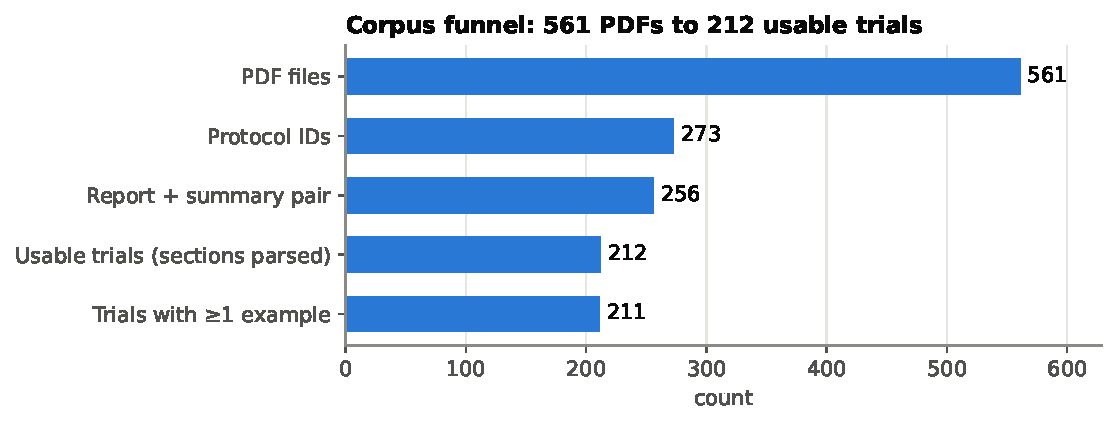
\includegraphics[width=\textwidth]{Figures/results/fig01_corpus_funnel.pdf}
    \caption[Corpus funnel]{From 561 PDFs to 212 usable trials.}
    \label{fig:funnel}
\end{figure}

\section{From Documents to Examples}

Each patient summary answers up to eight canonical patient questions. For every usable trial and question, an example is formed from the question, the report section(s) mapped to that question (the \emph{context}) and the patient-summary section that answers it (the \emph{reference}). The question-to-section mapping is the one defined in the original thesis. An example is dropped when the mapped report section is missing (\emph{no context}) or when the summary does not contain that question (\emph{no answer}).

Table~\ref{tab:coverage} and Figure~\ref{fig:coverage} give the coverage per question. The construction yields \textbf{959 examples}. Coverage is uneven: \emph{What were the results of the trial?} is answered for 201 trials, \emph{How has this trial helped?} for only 87. Most losses are \emph{no answer}, because older patient-summary templates do not ask every question.

\textbf{The adverse-events question contributes no examples.} Its mapped report section, \emph{Trial Analysis}, occurs in none of the 212 parsed reports. The same missing section leaves the treatments question with only \emph{Statistical Methods} as context and the results question with only \emph{Conclusion}. The study therefore evaluates \textbf{7 of the 8 questions}. This is a defect of the inherited mapping, not a property of the task: 179 of the patient summaries do answer the adverse-events question, and the reports contain safety sections that a corrected mapping could use (Section~\ref{sec:future}).

\begin{table}[htbp]
    \centering
    \small
    \caption[Examples per question]{Examples per question and reasons for exclusion (212 usable trials). The mapping of questions to report sections is inherited from the original thesis.}
    \label{tab:coverage}
    \begin{tabularx}{\textwidth}{>{\raggedright\arraybackslash}p{4.6cm}rrr>{\raggedright\arraybackslash}X}
        \toprule
        Question & Usable & No answer & No context & Mapped report sections \\
        \midrule
        \tabinput{Tables/dataset_coverage_body.tex}
        \bottomrule
    \end{tabularx}
\end{table}

\begin{figure}[htbp]
    \centering
    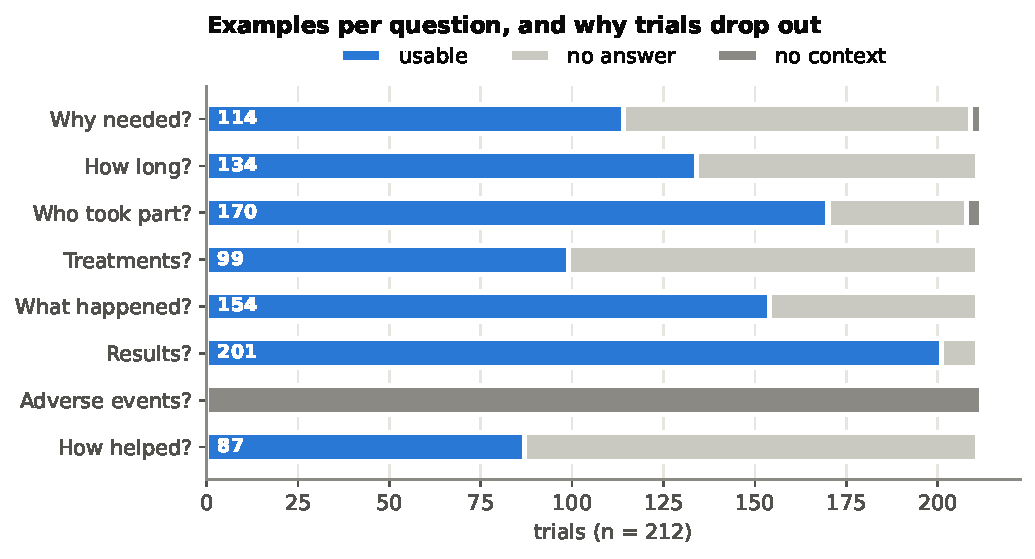
\includegraphics[width=\textwidth]{Figures/results/fig02_question_coverage.pdf}
    \caption[Coverage per question]{Examples per question and reasons for exclusion. The adverse-events question yields none because its mapped section is never extracted.}
    \label{fig:coverage}
\end{figure}

\section{Train, Validation and Test Split}

The examples are split \textbf{by trial} into 70/15/15 shares of the trials (seed 42), so that no trial contributes examples to two splits (Table~\ref{tab:splits}). The original thesis split 85/15 by row, which placed different questions about the same trial in both training and test data. The test set holds 138 examples from 31 trials; Table~\ref{tab:splits_q} gives the split per question. Per-question test cells contain between 12 and 28 examples, too few for claims about individual questions.

\begin{table}[htbp]
    \centering
    \begin{minipage}[t]{0.38\textwidth}
        \centering
        \caption[Dataset split]{Split by trial.}
        \label{tab:splits}
        \begin{tabular}{lrr}
            \toprule
            Split & Trials & Examples \\
            \midrule
            \tabinput{Tables/dataset_splits_body.tex}
            \bottomrule
        \end{tabular}
    \end{minipage}\hfill
    \begin{minipage}[t]{0.58\textwidth}
        \centering
        \caption[Split per question]{Examples per question and split.}
        \label{tab:splits_q}
        \begin{tabular}{lrrr}
            \toprule
            Question & Train & Val & Test \\
            \midrule
            \tabinput{Tables/dataset_splits_per_question_body.tex}
            \bottomrule
        \end{tabular}
    \end{minipage}
\end{table}

\section{How the Targets Differ from the Source}
\label{sec:targets}

Table~\ref{tab:textstats} and Figure~\ref{fig:src_ref} compare the references with their contexts over all 959 examples. Three contrasts define the task.

\begin{itemize}
    \item \textbf{The references are longer than their source.} The median reference has 183 words, the median context 136. Plain-language summarisation here is not compression: the patient summaries explain and expand, for example by defining terms. This matters for the metrics, because short outputs earn little recall.
    \item \textbf{The references are easier to read by the readability formulas.} The median Flesch--Kincaid grade falls from 15.10 in the report context to 10.03 in the references, and the median Flesch Reading Ease rises from 26.28 to 54.73. The source text is also far more variable (standard deviation of the grade 9.18 against 4.30), partly because some sections are tables or lists flattened to text, on which the formulas are unreliable.
    \item \textbf{The references are abstractive.} About 96\% of reference bigrams do not occur in the paired context (Figure~\ref{fig:abstractive}), and \textbf{none of the 959 references occurs verbatim in its context}.
\end{itemize}

The last point has a direct consequence for the extractive question-answering framing of the original thesis, discussed in Section~\ref{sec:extractive}.

\begin{table}[htbp]
    \centering
    \caption[Source vs. reference statistics]{Length, readability and abstractiveness of the report contexts and the plain-language references (all 959 examples). FKGL: Flesch--Kincaid grade level (lower is easier). Flesch Reading Ease: higher is easier.}
    \label{tab:textstats}
    \begin{tabular}{lrrr}
        \toprule
        Statistic & Mean & Median & SD \\
        \midrule
        \tabinput{Tables/dataset_text_stats_body.tex}
        \bottomrule
    \end{tabular}
\end{table}

\begin{figure}[htbp]
    \centering
    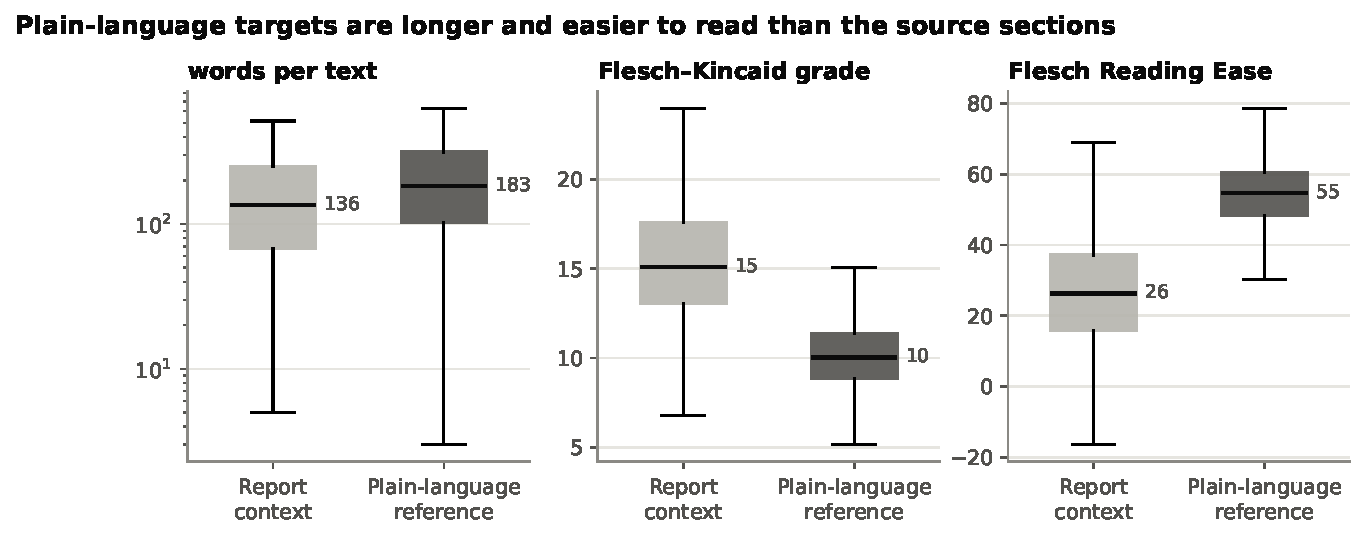
\includegraphics[width=\textwidth]{Figures/results/fig03_source_vs_reference.pdf}
    \caption[Source vs. reference]{Length and readability of report sections vs.\ plain-language references ($n = 959$).}
    \label{fig:src_ref}
\end{figure}

\begin{figure}[htbp]
    \centering
    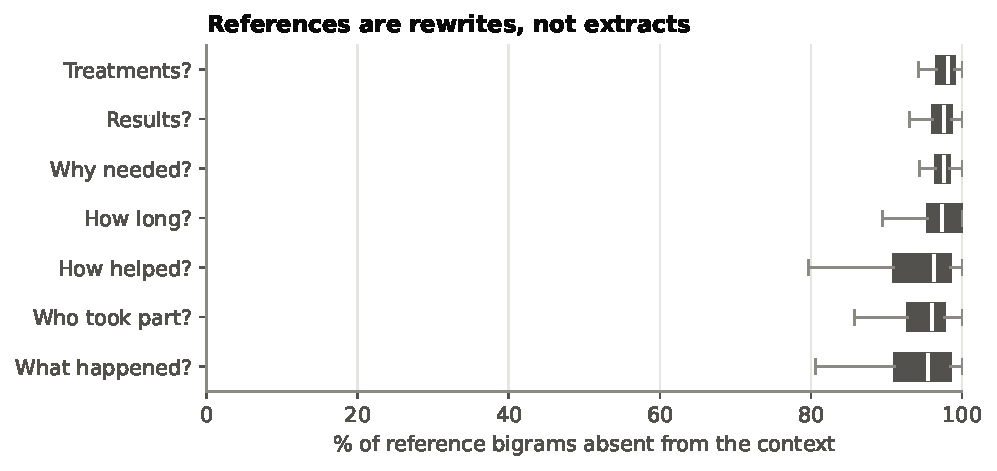
\includegraphics[width=0.85\textwidth]{Figures/results/fig04_reference_abstractiveness.pdf}
    \caption[Reference abstractiveness]{Share of reference bigrams absent from the source, per question.}
    \label{fig:abstractive}
\end{figure}
 
% Chapter 4

\chapter{Methods} % Main chapter title
\label{methods}

\section{Input Preparation}

Every system receives the same prompt, the one defined in the original thesis: the context, then the question, then an instruction to answer using only the context and in plain language. The context is capped at 900 Flan-T5 tokens so that the question, which follows the context, is never truncated away. The cap affected 4 of 138 test examples and 26 of 676 training examples. The input budget is 1024 tokens and the output (and training target) budget is 512 tokens. All systems are evaluated on the identical 138 test examples.

\section{Systems}

\begin{description}
    \item[Lead-$k$ ($k = 1, 2, 3$).] The first $k$ sentences of the context. These extractive baselines need no model.
    \item[DistilBERT-SQuAD.] The \nolinkurl{distilbert-base-cased-distilled-squad} checkpoint \parencite{sanh2019distilbert,rajpurkar2016squad}, used off the shelf. It extracts a span from the context and represents the extractive question-answering framing of the original thesis.
    \item[Flan-T5-small and Flan-T5-base, zero-shot.] The \texttt{google/flan-t5-small} and \texttt{-base} checkpoints \parencite{chung2024flan} without task training.
    \item[Qwen2.5-1.5B-Instruct, zero-shot.] A decoder-only instruction-tuned model \parencite{qwen2024qwen25}, run with its chat template in bfloat16. It is a CPU-feasible stand-in for the Mistral-7B-Instruct model of the original thesis, \emph{not} a reproduction of it.
    \item[Flan-T5-small, fully fine-tuned.] 5 epochs, learning rate $3\times10^{-4}$, batch size 4, fused AdamW, linear schedule without warm-up, weight decay 0, early stopping on validation loss with patience 2 (never triggered). Trained with seeds 42, 43 and 44.
    \item[Flan-T5-base with LoRA.] LoRA \parencite{hu2022lora} with rank $r = 8$, $\alpha = 8$, dropout 0, applied to the query and value projections; 3 epochs, learning rate $10^{-3}$, batch size 2, seed 42.
\end{description}

The training batch sizes were reduced from 8 (Flan-T5-small) and 4 (Flan-T5-base with LoRA) after a first attempt ran out of memory on the 15~GB machine. The LoRA configuration has a single seed and, as Appendix~\ref{sec:training} shows, was still improving when its budget ran out.

\section{Decoding}
\label{sec:decoding_protocol}

The main protocol is greedy decoding with \texttt{no\_repeat\_ngram\_size} $= 3$, which forbids any word-piece trigram from appearing twice in the generated text. Plain greedy decoding is reported as an ablation (Section~\ref{sec:decoding}). Greedy decoding replaces the temperature-0.7 sampling of the repository defaults, which is not reproducible.

For decoder-only models, the Hugging Face implementation of the no-repeat constraint also scans the prompt, so it forbids copying any trigram of the source. We restricted the constraint to generated tokens, which matches its behaviour for encoder-decoder models. The superseded Qwen run with the prompt-scanning behaviour is kept with the results for transparency but not reported.

\section{Metrics}
\label{sec:metrics}

All overlap and semantic metrics are reported on a 0--100 scale.

\begin{itemize}
    \item \textbf{Overlap metrics:} ROUGE-1, ROUGE-2 and ROUGE-L F1 with stemming \parencite{lin2004rouge}; sentence-level BLEU \parencite{papineni2002bleu} with smoothing method 4 \parencite{chen2014smoothing}; and token F1 after SQuAD-style normalisation \parencite{rajpurkar2016squad}. Exact match is 0 for every system, because no output reproduces a free-text reference exactly, so it is omitted.
    \item \textbf{BERTScore-F1} \parencite{zhang2020bertscore} with \texttt{roberta-large} and \textbf{baseline rescaling}. Rescaling places the score of unrelated text pairs near zero, so negative values are expected for weak systems and are not an error.
    \item \textbf{Readability:} Flesch--Kincaid grade level (FKGL) \parencite{kincaid1975} and Flesch Reading Ease \parencite{flesch1948}, computed with \texttt{textstat}. Readability is computed only for outputs of at least three words.
    \item \textbf{Faithfulness proxies.} \emph{Number support} is the share of numbers in an output that also appear in the context. \emph{Code support} is the same for drug and protocol codes such as ACZ885. A number or code absent from the context is a candidate unsupported detail. Both are string-matching signals, not factuality judgements: they ignore non-numeric claims and can miss a correct number written in another format.
    \item \textbf{Abstractiveness:} the share of output bigrams that do not occur in the context (\emph{novel bigrams}).
    \item \textbf{Repetition:} the share of repeated word trigrams in an output. An output counts as repetitive when this share exceeds 0.2.
\end{itemize}

\section{Statistical Analysis}

Examples from the same trial are correlated, so a per-example bootstrap would give intervals that are too narrow. We therefore report 95\% confidence intervals from a \textbf{cluster bootstrap over trials} \parencite{efron1994bootstrap} with 2000 resamples (seed 42). Pairs of systems are compared with paired Wilcoxon signed-rank tests \parencite{wilcoxon1945} on per-example differences, with Holm correction \parencite{holm1979} over the family of 20 comparisons (10 system pairs, two metrics each). As effect sizes we report the mean difference with its trial-level confidence interval and the share of examples on which the first system scores higher. With 138 examples, very small $p$-values say little about practical importance, so the discussion relies on the effect sizes.

\section{Compute and Software}

All experiments ran on a CPU-only machine (8 cores, 15~GB RAM, WSL2) without a GPU. Each fine-tuning run took between 93.8 and 99.6 minutes (Appendix~\ref{sec:cost}). Software versions: Python 3.14.4, PyTorch 2.14.1, Transformers 5.19.0 \parencite{wolf2020transformers}, PEFT 0.21.2, rouge-score 0.1.2, NLTK 3.10.3, bert-score 0.3.13 and textstat 0.7.13. Appendix~\ref{sec:repro} lists where this protocol deviates from the repository defaults.
 
% Chapter 5

\chapter{Results} % Main chapter title
\label{results}

All results are on the test set (138 examples from 31 held-out trials) under the main decoding protocol unless stated otherwise.

\section{Main Comparison}

Table~\ref{tab:main} gives the mean scores of every system and Figure~\ref{fig:main} shows them with 95\% trial-level confidence intervals. Appendix Tables~\ref{tab:main_ci_a} and~\ref{tab:main_ci_b} list all intervals.

\begin{table}[htbp]
    \centering
    \small
    \caption[Main results]{Test-set scores under the main protocol (greedy decoding with no-repeat-3; 138 examples, 31 trials). BERTScore is baseline-rescaled, so negative values are expected. Best value per column in bold. FT: fine-tuned; s42--s44: training seeds.}
    \label{tab:main}
    \resizebox{\textwidth}{!}{%
    \begin{tabular}{lrrrrrr}
        \toprule
        System & ROUGE-1 & ROUGE-2 & ROUGE-L & BLEU & Token F1 & BERTScore \\
        \midrule
        \tabinput{Tables/main_results_body.tex}
        \bottomrule
    \end{tabular}}
\end{table}

\begin{figure}[htbp]
    \centering
    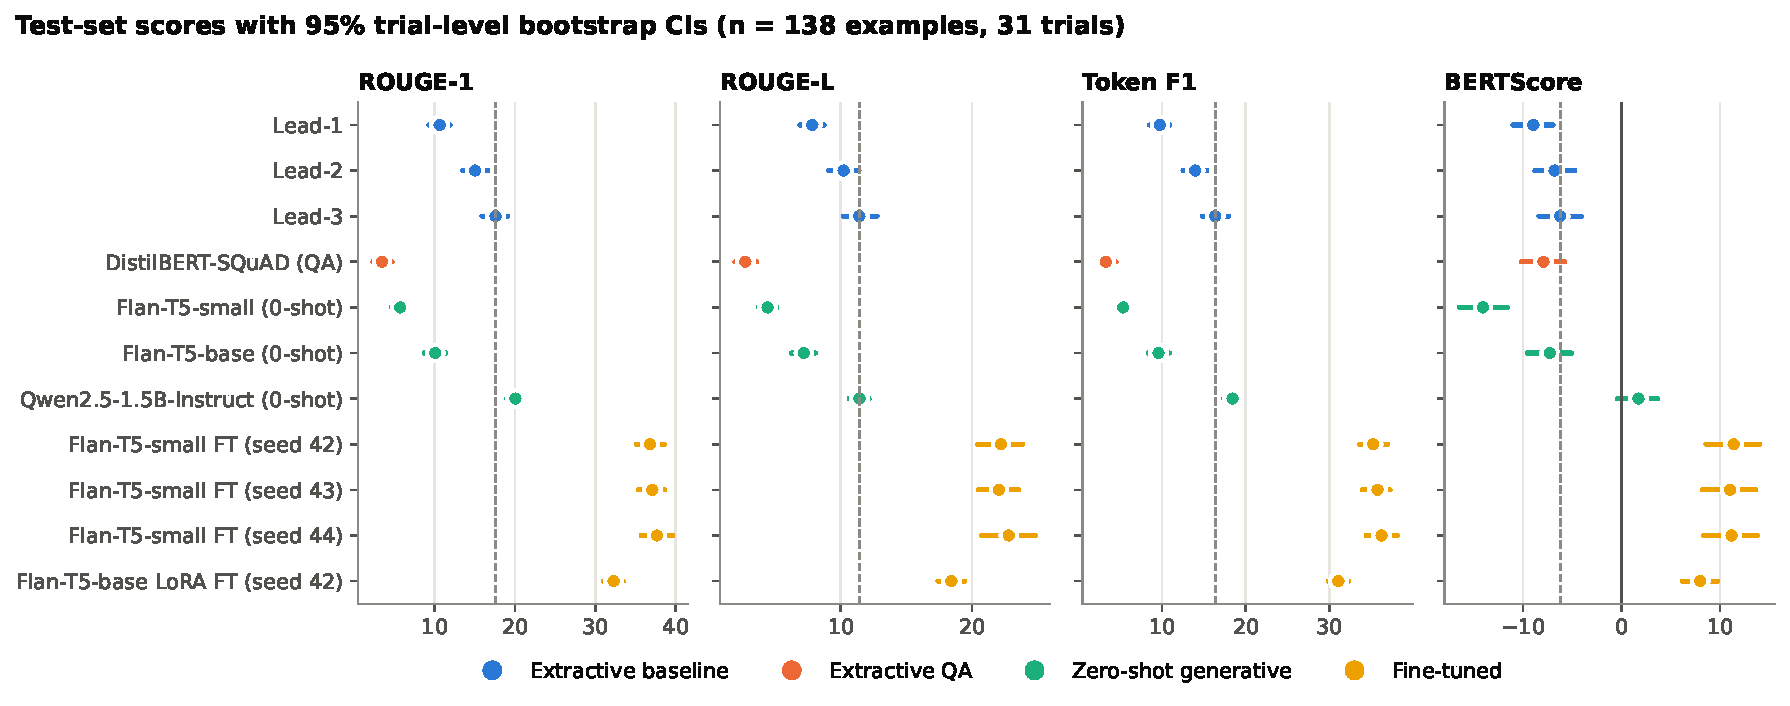
\includegraphics[width=\textwidth]{Figures/results/fig05_main_results_ci.pdf}
    \caption[Main results with confidence intervals]{Test-set scores with 95\% trial-level bootstrap CIs (138 examples, 31 trials). Dashed line: Lead-3.}
    \label{fig:main}
\end{figure}

\paragraph{Fine-tuning dominates on every automatic metric.} After fine-tuning, Flan-T5-small reaches a ROUGE-L of 22.36 $\pm$ 0.39 (mean $\pm$ standard deviation over three seeds), roughly double that of Lead-3 (11.41), the strongest simple baseline. Its BERTScore is 11.21 $\pm$ 0.18, against $-$6.22 for Lead-3. The confidence intervals of the fine-tuned models overlap with no baseline or zero-shot system on any of the metrics shown in Figure~\ref{fig:main}.

\paragraph{Training noise is small.} Table~\ref{tab:seeds} gives the seed variance of fine-tuned Flan-T5-small. The standard deviation across seeds (0.39 ROUGE-L, 0.18 BERTScore) is an order of magnitude smaller than the gaps between system families. Seed variance was measured only for this configuration; the LoRA model has a single seed.

\begin{table}[htbp]
    \centering
    \small
    \caption[Seed variance]{Seed variance of fine-tuned Flan-T5-small (mean $\pm$ standard deviation over seeds 42, 43 and 44).}
    \label{tab:seeds}
    \resizebox{\textwidth}{!}{%
    \begin{tabular}{lrrrrrr}
        \toprule
        System & ROUGE-1 & ROUGE-2 & ROUGE-L & BLEU & Token F1 & BERTScore \\
        \midrule
        \tabinput{Tables/seed_variance_body.tex}
        \bottomrule
    \end{tabular}}
\end{table}

\paragraph{The smaller, fully fine-tuned model beats LoRA on the base model, under our budget.} Flan-T5-base with LoRA reaches a ROUGE-L of 18.43 and a BERTScore of 8.00, below every Flan-T5-small seed. This holds only for our CPU budget: the LoRA run has one seed and its validation loss was still falling after three epochs (Appendix~\ref{sec:training}). It is not evidence that larger models are worse.

\paragraph{Zero-shot systems are weak, and Qwen ties Lead-3 on ROUGE-L.} Qwen2.5-1.5B-Instruct ties Lead-3 on ROUGE-L (11.43 against 11.41) but is clearly ahead on BERTScore (1.73 against $-$6.22): it paraphrases rather than copies, without matching the wording of the references. Zero-shot Flan-T5 scores below Lead-1 on ROUGE-L (4.43 for the small and 7.19 for the base model, against 7.83), largely because its outputs are very short (Section~\ref{sec:length}).

\paragraph{Extractive question answering is the weakest system.} DistilBERT-SQuAD reaches a ROUGE-L of 2.72 and returns an empty answer for 40.6\% of the test examples. Section~\ref{sec:extractive} explains why.

\section{Paired Tests}

Table~\ref{tab:paired} reports the paired comparisons. Every comparison is significant after Holm correction except two. \textbf{Qwen and Lead-3 do not differ on ROUGE-L} (mean difference 0.01 [$-$0.94, 0.84], $p_\text{Holm} = 0.660$) although Qwen is ahead on BERTScore by 7.95 [6.63, 9.19]. \textbf{DistilBERT-SQuAD and Lead-3 do not differ on BERTScore} ($p_\text{Holm} = 0.660$), while DistilBERT is far behind on ROUGE-L. Fine-tuned Flan-T5-small beats Lead-3 by 10.81 [9.61, 12.01] ROUGE-L, scoring higher on 94.2\% of examples, and by 17.61 [15.13, 20.19] BERTScore, scoring higher on 87.0\%. Fine-tuning adds 17.79 ROUGE-L and 25.46 BERTScore to zero-shot Flan-T5-small, and 11.24 and 15.29 to zero-shot Flan-T5-base. Flan-T5-base with LoRA trails fine-tuned Flan-T5-small by 3.79 [2.65, 4.92] ROUGE-L and 3.39 [0.97, 5.48] BERTScore ($p_\text{Holm} = 0.004$).

\begin{table}[htbp]
    \centering
    \footnotesize
    \caption[Paired tests]{Paired comparisons on the 138 test examples. $\Delta$: mean per-example difference (A $-$ B) with 95\% trial-level CI. Win\,\%: share of examples on which A scores higher. $p$: Wilcoxon signed-rank, Holm-corrected over all 20 comparisons. Systems use the main protocol unless marked ``plain greedy''.}
    \label{tab:paired}
    \resizebox{\textwidth}{!}{%
    \begin{tabular}{lrrrrrr}
        \toprule
        & \multicolumn{3}{c}{ROUGE-L} & \multicolumn{3}{c}{BERTScore} \\
        \cmidrule(lr){2-4}\cmidrule(lr){5-7}
        A vs B & $\Delta$ [95\% CI] & Win\,\% & $p$ & $\Delta$ [95\% CI] & Win\,\% & $p$ \\
        \midrule
        \tabinput{Tables/paired_tests_body.tex}
        \bottomrule
    \end{tabular}}
\end{table}

\section{Decoding Ablation}
\label{sec:decoding}

Table~\ref{tab:decoding} and Figure~\ref{fig:decoding} compare plain greedy decoding with the main protocol. The inputs and models are identical; only the decoding rule changes.

\begin{table}[htbp]
    \centering
    \footnotesize
    \caption[Decoding ablation]{Decoding ablation on the test set. PG: plain greedy. NR3: greedy with no-repeat-3 (main protocol). Rep.\,\%: share of outputs with more than 20\% repeated word trigrams. Code and number support: share of codes or numbers in the output found in the context.}
    \label{tab:decoding}
    \resizebox{\textwidth}{!}{%
    \begin{tabular}{lrrrrrrrrrr}
        \toprule
        & \multicolumn{2}{c}{ROUGE-L} & \multicolumn{2}{c}{BERTScore} & \multicolumn{2}{c}{Rep.\,\%} & \multicolumn{2}{c}{Code support} & \multicolumn{2}{c}{Number support} \\
        \cmidrule(lr){2-3}\cmidrule(lr){4-5}\cmidrule(lr){6-7}\cmidrule(lr){8-9}\cmidrule(lr){10-11}
        System & PG & NR3 & PG & NR3 & PG & NR3 & PG & NR3 & PG & NR3 \\
        \midrule
        \tabinput{Tables/decoding_ablation_body.tex}
        \bottomrule
    \end{tabular}}
\end{table}

\begin{figure}[htbp]
    \centering
    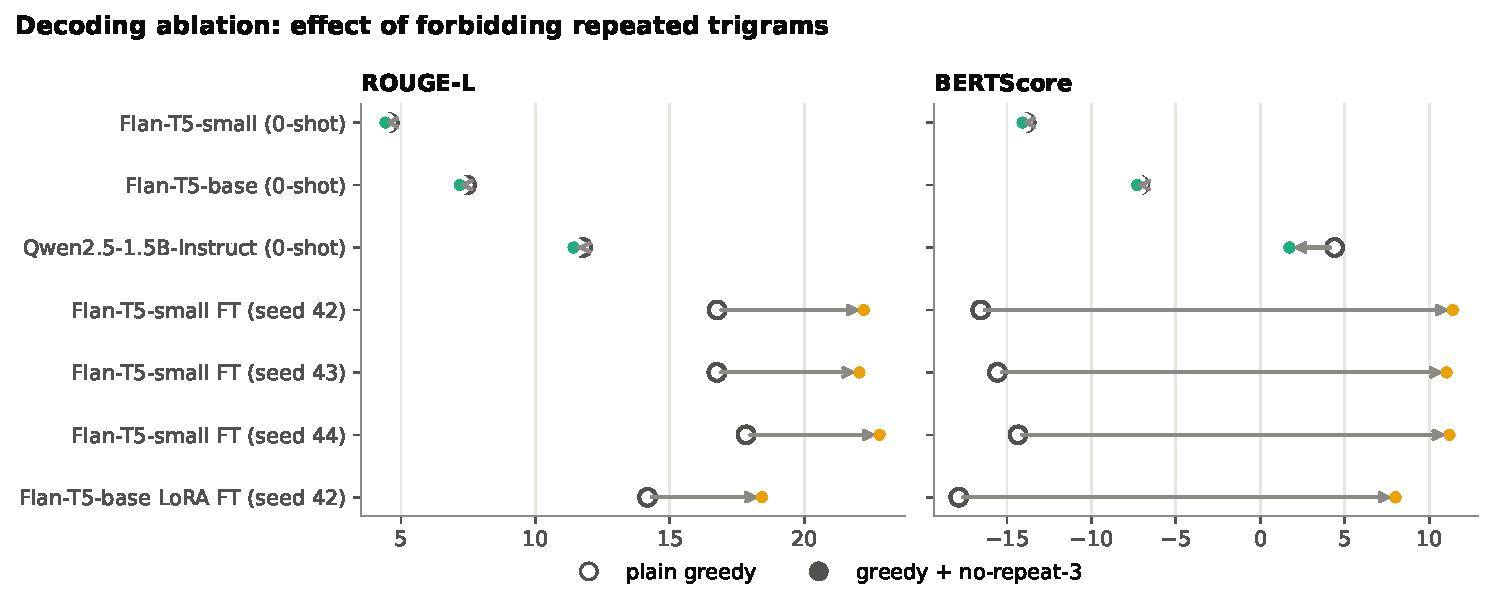
\includegraphics[width=\textwidth]{Figures/results/fig11_decoding_ablation.pdf}
    \caption[Decoding ablation]{Effect of forbidding repeated trigrams (open circle: plain greedy; filled: no-repeat-3).}
    \label{fig:decoding}
\end{figure}

\paragraph{Plain greedy decoding makes the fine-tuned models loop.} Between 86.23\% and 89.13\% of the fine-tuned Flan-T5-small outputs, and 98.55\% of the LoRA outputs, are repetitive. Yet under plain greedy decoding fine-tuned Flan-T5-small (seed 42) still scores a ROUGE-L of 16.76, above Lead-3, while its BERTScore of $-$16.54 is lower than that of every system in the main table. \textbf{ROUGE alone would have reported a working system.} Looping text keeps reusing domain vocabulary that also occurs in the reference, which feeds unigram and longest-common-subsequence overlap.

\paragraph{The no-repeat constraint removes the loops but is not free.} It brings the share of repetitive outputs to 0 and raises BERTScore by 27.94 for fine-tuned Flan-T5-small and 25.85 for LoRA, and ROUGE-L by 5.46 and 4.26 (Table~\ref{tab:paired}). But it also prevents the model from writing the same multi-token drug code twice. Code support of the fine-tuned models falls from 0.95--1.00 under plain greedy decoding to 0.35--0.46: the second mention of a code mutates, for example ACZ885 becomes ACZ855.

\paragraph{Zero-shot models are barely affected,} because they did not loop in the first place. Qwen does slightly better under plain greedy decoding (BERTScore 4.40 against 1.73).

Together with the Qwen and Lead-3 tie, the ablation shows that \textbf{the conclusion a metric supports depends on decoding settings and on the choice of metric}. Decoding settings should be reported as part of the system definition, and overlap metrics should be accompanied by a semantic metric and a repetition check.

% Chapter 6

\chapter{Analysis and Discussion} % Main chapter title
\label{analysis}

\section{Per-Question Performance}

Table~\ref{tab:perq} and Figure~\ref{fig:perq} break ROUGE-L down by question. Each cell averages only 12 to 28 examples, so we read patterns across rows rather than individual cells.

\begin{table}[htbp]
    \centering
    \footnotesize
    \caption[ROUGE-L per question]{ROUGE-L per question on the test set (main protocol). Each cell averages 12--28 examples.}
    \label{tab:perq}
    \resizebox{\textwidth}{!}{%
    \begin{tabular}{lrrrrrrr}
        \toprule
        \tabinput{Tables/per_question_head.tex}
        \midrule
        \tabinput{Tables/per_question_body.tex}
        \bottomrule
    \end{tabular}}
\end{table}

\begin{figure}[htbp]
    \centering
    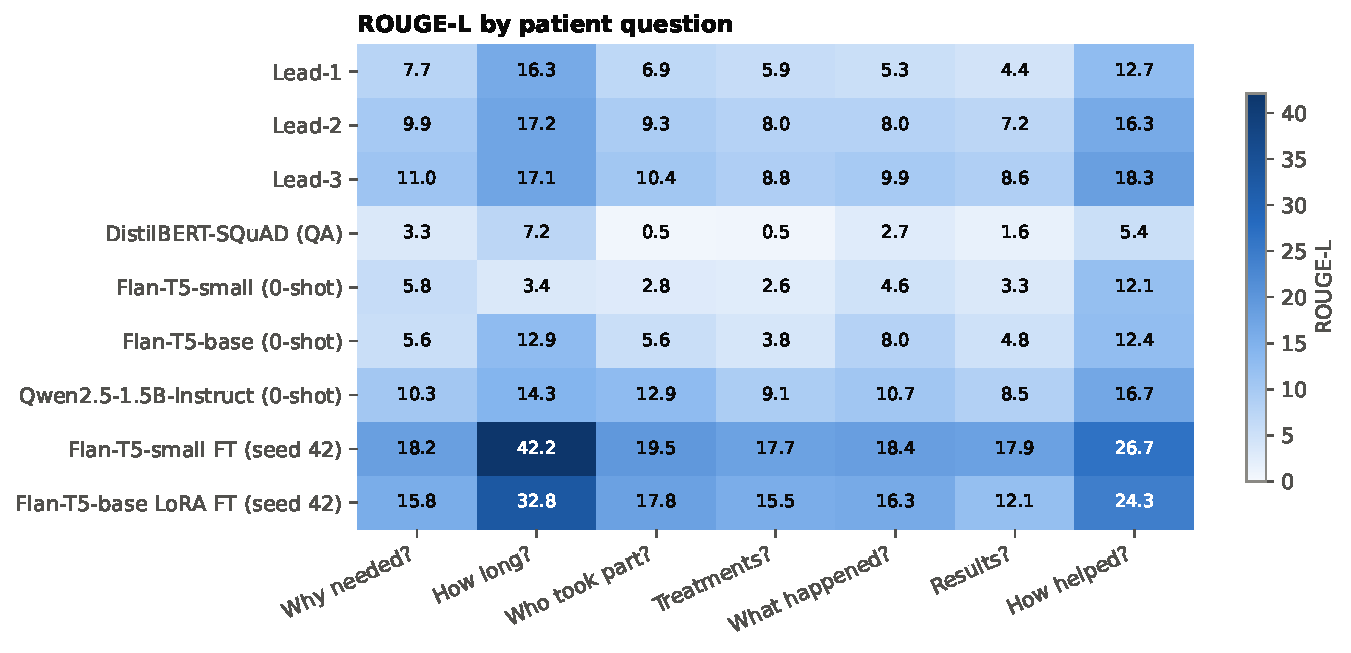
\includegraphics[width=\textwidth]{Figures/results/fig06_per_question_rougeL.pdf}
    \caption[ROUGE-L by question]{ROUGE-L by question.}
    \label{fig:perq}
\end{figure}

\emph{How long was the trial?} is the easiest question for the trained systems (fine-tuned Flan-T5-small: 42.2). Its answers are formulaic and the dates are present in the context. \emph{Results} and \emph{Treatments} are among the hardest for every system, which is consistent with the mapping defect described in Chapter~\ref{data}: these questions are answered only from the \emph{Conclusion} and \emph{Statistical Methods} sections respectively, so most of what the reference conveys is missing from the input. Fine-tuned Flan-T5-small has the highest ROUGE-L on all seven questions.

\section{Length and Readability of the Outputs}
\label{sec:length}

Table~\ref{tab:props} and Figure~\ref{fig:length} compare the outputs with the human references. Three groups emerge, and only the fine-tuned models resemble the references in both length and reading level.

\begin{table}[htbp]
    \centering
    \footnotesize
    \caption[Output properties]{Properties of the outputs on the test set (means; main protocol). FKGL: Flesch--Kincaid grade level. Novel bigrams: share of output bigrams absent from the context. Number and code support: share of numbers or drug/protocol codes in the output found in the context. Empty: share of empty outputs (\%).}
    \label{tab:props}
    \resizebox{\textwidth}{!}{%
    \begin{tabular}{lrrrrrrr}
        \toprule
        & Words & FKGL & Flesch & Novel bigrams & Number support & Code support & Empty \% \\
        \midrule
        \tabinput{Tables/output_properties_body.tex}
        \bottomrule
    \end{tabular}}
\end{table}

\begin{figure}[htbp]
    \centering
    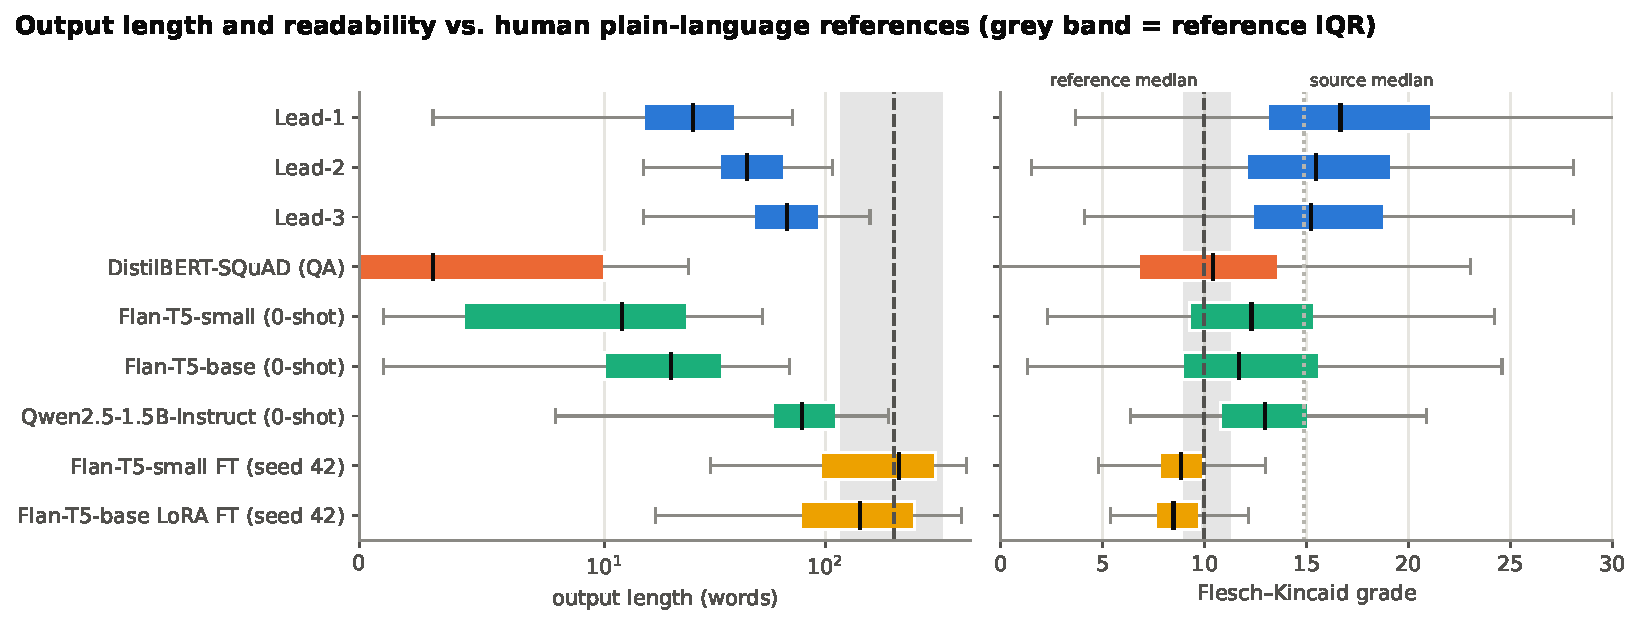
\includegraphics[width=\textwidth]{Figures/results/fig07_length_readability.pdf}
    \caption[Length and readability of outputs]{Output length and FKGL vs.\ the human references (grey band: reference interquartile range).}
    \label{fig:length}
\end{figure}

\begin{itemize}
    \item \textbf{Extractive systems} copy technical text and inherit its difficulty: Lead-3 has a mean FKGL of 17.57 and a Flesch score of 22.7.
    \item \textbf{Zero-shot generators are too short.} Zero-shot Flan-T5 outputs have a median of 12 (small) and 20 (base) words; Qwen's median is 78 words. Their FKGL (12.02 to 13.09) is lower than that of the source but higher than that of the references.
    \item \textbf{Fine-tuned models match the reference profile.} Fine-tuned Flan-T5-small has a mean FKGL of 9.28 against 10.27 for the human references, and a Flesch score of 57.8 against 54.9; LoRA is similar (9.24 and 58.2).
\end{itemize}

Fine-tuning therefore mainly teaches the \emph{register and length} of patient summaries. That alone accounts for part of the gain in overlap metrics, because length-matched outputs earn recall that short outputs cannot. The readability formulas measure only sentence and word length; a lower FKGL does not show that a text is good plain language, let alone that it is correct.

\section{Abstractiveness and Faithfulness Proxies}
\label{sec:faithfulness}

Figure~\ref{fig:faith} plots how much each system rewrites (novel bigrams) against the share of its numbers found in the source (number support). The ideal plain-language system would sit top right: it rewrites like the references without stating numbers the source does not support.

\begin{figure}[htbp]
    \centering
    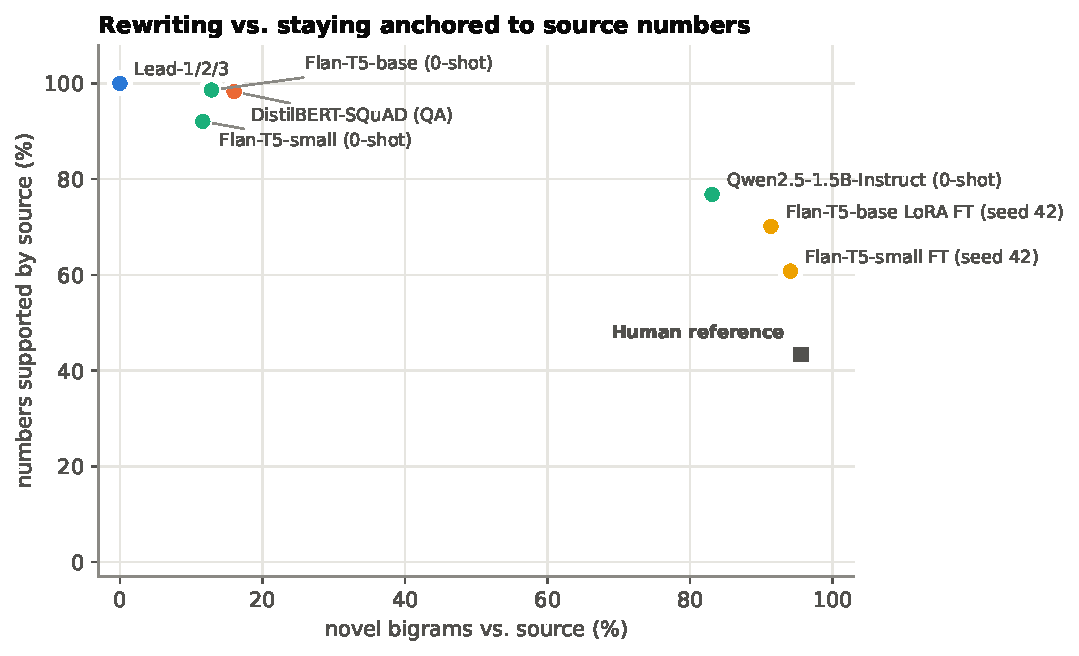
\includegraphics[width=0.85\textwidth]{Figures/results/fig08_abstractiveness_vs_faithfulness.pdf}
    \caption[Abstractiveness vs. number support]{Rewriting (novel bigrams) vs.\ numbers supported by the source. The grey square marks the human references.}
    \label{fig:faith}
\end{figure}

The horizontal axis separates copiers from rewriters. Lead-$k$, DistilBERT-SQuAD and zero-shot Flan-T5 rewrite little (novel-bigram shares of 0.00 to 0.16); Qwen (0.83) and the fine-tuned models (0.91 and 0.94) rewrite almost as much as the references (0.96).

The vertical axis needs care, because \textbf{the human references themselves have a number support of only 0.43 and a code support of 0.53}. Most numbers in a reference do not appear in its mapped context: the patient summaries draw on parts of the report that the question-to-section mapping does not provide. The input is under-specified for the target. The fine-tuned models sit between the copiers and the references, with number support of 0.61 (Flan-T5-small) and 0.70 (LoRA).

\emph{Interpretation.} Because the references contain details absent from the mapped input, models trained to imitate them are rewarded for producing such details. We read this as a property of the dataset construction, not only of the models, and we treat it as a moderate claim: it rests on a string-matching proxy, and the references are not ground truth for every fact. Number and code support do not measure factuality.

\section{A Typical Example}
\label{sec:example}

To illustrate what the scores hide, we inspect one test example: the question \emph{Why was the research needed?} for trial CAIN457H3301. It was chosen as the example whose fine-tuned Flan-T5-small ROUGE-L is closest to that model's median, so it is typical rather than selected for effect. Data licensing limits quotation to short fragments.

\begin{itemize}
    \item \textbf{Lead-3 and DistilBERT-SQuAD} copy the trial objective verbatim. This is accurate but not plain language.
    \item \textbf{Qwen} gives a correct but more technical paraphrase that keeps clinical jargon such as the BASDAI score (ROUGE-L 7.5, BERTScore $-$8.2).
    \item \textbf{Fine-tuned Flan-T5-small} reproduces the opening of the reference almost word for word (``Researchers are looking for a better way to treat\ldots''), then degrades into garbled terms such as ``sapondyritis'' and a misspelt drug name, ``scukinumab''. It has the highest ROUGE-L of all systems on this example (19.5) and the second-highest BERTScore ($-$5.4).
    \item \textbf{Flan-T5-base with LoRA} has the highest BERTScore on the example ($-$1.9) but introduces conditions the source does not mention, such as an ``active bladder infection'' and a drug ``used to treat septicemia''.
\end{itemize}

On this example the automatic metrics rank the outputs by stylistic similarity to the reference, not by correctness; the output a patient could most safely read comes from the zero-shot Qwen model, which scores lower on both metrics.

\section{Why Extractive Question Answering Does Not Fit}
\label{sec:extractive}

No reference occurs verbatim in its source section (Section~\ref{sec:targets}), so span-extraction labels are undefined for every example. In the original pipeline, span labels were computed by searching for the answer string in the context; this search fails for all 959 examples, and every training label collapses to the ``no answer'' position. Empirically, the off-the-shelf DistilBERT-SQuAD model is the weakest system in the study (ROUGE-L 2.72) and returns an empty answer for 40.6\% of the test examples. The task is abstractive by construction, and an extractive model cannot in principle reproduce its targets.

\section{Answers to the Research Questions}

\paragraph{RQ1: Can small CPU-trainable models match human summaries better than the baselines?} By every automatic metric, yes. Fine-tuned Flan-T5-small reaches a ROUGE-L of 22.36 $\pm$ 0.39 over three seeds, roughly double that of Lead-3 (11.41), with non-overlapping confidence intervals and Holm-corrected paired tests, and it matches the references in length and readability (FKGL 9.28 against 10.27). Each fine-tuning run took about one and a half hours on a CPU. This answer concerns similarity to the references, not correctness (RQ4).

\paragraph{RQ2: Does the extractive QA framing suit the task?} No. No reference is a substring of its context, so span labels are undefined, and the extractive model is the weakest system.

\paragraph{RQ3: How sensitive are the conclusions to decoding and metric choice?} Highly. Under plain greedy decoding, ROUGE ranks a model that loops in 86\% of its outputs above Lead-3, while BERTScore ranks it below every system in the main table. Under the main protocol, Qwen ties Lead-3 on ROUGE-L but is clearly ahead on BERTScore.

\paragraph{RQ4: Do automatic metrics reflect faithfulness?} The evidence so far suggests not. Qualitative inspection and string-level faithfulness proxies suggest that the automatic metrics reward the style of patient summaries more than their correctness: the systems that win every metric produce garbled or unsupported content on a typical example, and the references themselves contain many numbers and codes absent from the input. This claim is of moderate strength. It rests on proxies and one systematically chosen example; the planned human evaluation (Section~\ref{sec:limitations}) is needed to confirm or reject it.

No system in this study produces summaries that can be considered factually reliable or safe for patients without human review.

% Chapter 7

\chapter{Limitations, Future Work and Conclusions} % Main chapter title
\label{conclusion}

\section{Limitations}
\label{sec:limitations}

The limitations are listed in order of importance.

\begin{enumerate}
    \item \textbf{No human evaluation.} The faithfulness evidence consists of string-level proxies and one qualitative example. A blinded human evaluation has been prepared (30 test examples, four systems, 120 items, rated for unsupported claims, completeness and plainness against the model input) but not yet carried out. Until it is, the claim that the metrics reward style rather than correctness remains of moderate strength.
    \item \textbf{The question-to-section mapping is inherited and defective.} One question yields no examples, two others receive only part of the relevant report, and the references contain information absent from the input.
    \item \textbf{Single test split.} The test set has 31 trials and 138 examples. The confidence intervals reflect this, but there is no cross-validation.
    \item \textbf{Compute.} All work ran on a CPU. The LoRA configuration has one seed and was under-trained within its budget, and no model of the 7-billion-parameter scale of the original thesis was run.
    \item \textbf{Metric caveats.} The $n$-gram metrics and BERTScore measure similarity to a single reference, and the references are not ground truth for every fact.
    \item \textbf{Decoding trade-off.} The no-repeat constraint removes loops but corrupts legitimately repeated entities such as drug codes.
    \item \textbf{Corpus.} All documents come from one sponsor (Novartis) and are in English. 44 trials were lost to PDF parsing failures.
    \item \textbf{Minor non-determinism in ingestion.} Three of the 959 examples differed in token order between two runs of the same pipeline.
\end{enumerate}

\section{Future Work}
\label{sec:future}

\begin{itemize}
    \item \textbf{Fix the data.} Map the adverse-events question to the safety sections of the reports, which would add about 179 examples, and give models the full report rather than single sections, so that the input supports the references.
    \item \textbf{Measure faithfulness directly.} Complete the human evaluation and add QA-based \parencite{wang2020qags} or NLI-based \parencite{laban2022summac} consistency metrics.
    \item \textbf{Better decoding.} Prevent loops without blocking legitimate repeats, for example with contrastive search \parencite{su2022contrastive} or a repetition penalty that exempts tokens copied from the source.
    \item \textbf{More compute.} Train on GPUs with larger models, more seeds and longer LoRA training.
\end{itemize}

\section{Conclusions}

This thesis rebuilt the plain-language summarisation dataset of the original study from 561 Novartis clinical-trial PDFs, obtaining 959 question-level examples from 212 usable trials, split by trial. On a held-out test set of 31 trials, fine-tuned Flan-T5-small improves every automatic metric by a wide margin over extractive and zero-shot baselines and matches the length and readability of human patient summaries, using only a CPU.

The evaluation also shows why these numbers should not be read as quality. The extractive question-answering framing of the original thesis cannot work on this data, because no reference occurs in its source. Decoding settings alone can make ROUGE endorse looping output. And qualitative inspection together with string-level proxies suggests that the metrics reward the register of patient summaries rather than their correctness, a tendency the dataset construction reinforces by pairing references with inputs that do not contain all of their facts. Generating plain-language summaries of clinical trials that patients can trust will need better-specified inputs, direct measurement of faithfulness, and human evaluation.




%----------------------------------------------------------------------------------------
%	THESIS CONTENT - APPENDICES
%----------------------------------------------------------------------------------------

\appendix % Cue to tell LaTeX that the following "chapters" are Appendices

% Include the appendices of the thesis as separate files from the Appendices folder
% Uncomment the lines as you write the Appendices

% Appendix A

\chapter{Supporting Results and Reproducibility} % Main appendix title
\label{AppendixA}

\section{Confidence Intervals for the Main Results}

Tables~\ref{tab:main_ci_a} and~\ref{tab:main_ci_b} give every main-table score with its 95\% cluster-bootstrap confidence interval over trials (2000 resamples).

\begin{table}[htbp]
    \centering
    \small
    \caption[Main results with CIs: ROUGE]{ROUGE scores with 95\% trial-level CIs (test set, main protocol).}
    \label{tab:main_ci_a}
    \resizebox{\textwidth}{!}{%
    \begin{tabular}{llll}
        \toprule
        System & ROUGE-1 & ROUGE-2 & ROUGE-L \\
        \midrule
        \tabinput{Tables/main_results_ci_overlap_body.tex}
        \bottomrule
    \end{tabular}}
\end{table}

\begin{table}[htbp]
    \centering
    \small
    \caption[Main results with CIs: BLEU, token F1, BERTScore]{BLEU, token F1 and BERTScore with 95\% trial-level CIs (test set, main protocol). BERTScore is baseline-rescaled.}
    \label{tab:main_ci_b}
    \resizebox{\textwidth}{!}{%
    \begin{tabular}{llll}
        \toprule
        System & BLEU & Token F1 & BERTScore \\
        \midrule
        \tabinput{Tables/main_results_ci_other_body.tex}
        \bottomrule
    \end{tabular}}
\end{table}

\section{Training Dynamics}
\label{sec:training}

Figure~\ref{fig:loss} shows the validation loss (145 examples, 32 trials) after every epoch. It falls monotonically for every run, and early stopping never triggered, so training was budget-limited rather than converged. The three Flan-T5-small seeds trace almost identical curves, with final losses between 1.920 and 1.927. Flan-T5-base with LoRA ends at 2.102 after three epochs, higher than the small model's loss after two epochs, and is still decreasing: within the CPU budget it was under-trained. Validation loss is token-level cross-entropy under teacher forcing and does not reveal decoding pathologies such as the repetition loops of Section~\ref{sec:decoding}, which occurred at the lowest-loss checkpoints.

\begin{figure}[htbp]
    \centering
    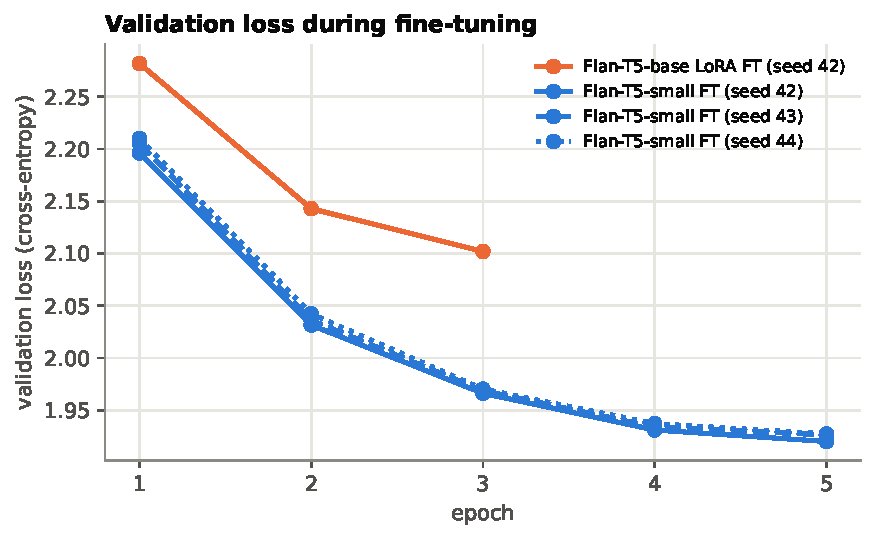
\includegraphics[width=0.85\textwidth]{Figures/results/fig09_validation_loss.pdf}
    \caption[Validation loss]{Validation loss per epoch.}
    \label{fig:loss}
\end{figure}

\section{Compute Cost}
\label{sec:cost}

Table~\ref{tab:cost} gives the median wall-clock generation time per test example (model loading excluded) and the training time. Fine-tuned outputs take longer to generate than zero-shot ones mainly because they are much longer.

\begin{table}[htbp]
    \centering
    \small
    \caption[Compute cost]{Compute cost on the CPU-only machine (8 cores, 15~GB RAM). Latency: median generation time per test example under the main protocol.}
    \label{tab:cost}
    \begin{tabular}{lrrr}
        \toprule
        System & Latency (s) & Training (min) & Epochs \\
        \midrule
        \tabinput{Tables/compute_cost_body.tex}
        \bottomrule
    \end{tabular}
\end{table}

\section{Retrieval Quality of the RAG Index}

The project also contains a retrieval-augmented generation (RAG) layer, which is not part of the summarisation experiments. Its index chunks the report sections of all 212 trials and embeds them with a dependency-free hashing embedder. For each of the 959 (trial, question) pairs, a chunk counts as relevant if it comes from a report section mapped to that question, and retrieval is restricted to the trial. Table~\ref{tab:rag} and Figure~\ref{fig:rag} show that retrieval with this embedder is weak (recall@5 of 0.275, mean reciprocal rank of 0.211), and precision@$k$ stays near 0.10 for every $k$. The relevance labels inherit the question-to-section mapping, so they cover only the seven answerable questions.

\begin{table}[htbp]
    \centering
    \small
    \caption[RAG retrieval]{Retrieval quality of the RAG index (959 queries, retrieval scoped to the trial).}
    \label{tab:rag}
    \begin{tabular}{rrrr}
        \toprule
        $k$ & Recall@$k$ & Precision@$k$ & MRR \\
        \midrule
        \tabinput{Tables/rag_body.tex}
        \bottomrule
    \end{tabular}
\end{table}

\begin{figure}[htbp]
    \centering
    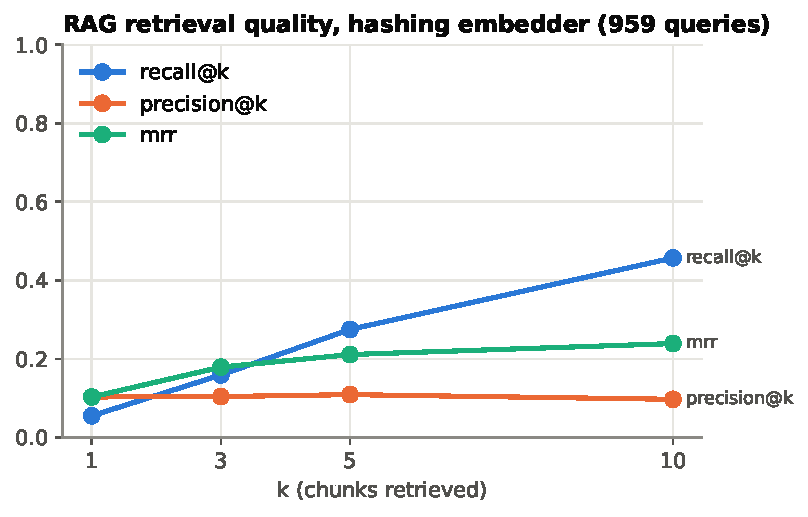
\includegraphics[width=0.7\textwidth]{Figures/results/fig10_rag_retrieval.pdf}
    \caption[RAG retrieval]{Retrieval quality of the RAG index.}
    \label{fig:rag}
\end{figure}

\section{Deviations from the Repository Defaults}
\label{sec:repro}

The experiments use the project's own pipeline, with the changes in Table~\ref{tab:deviations}. The scripts, logs, per-example outputs and notebooks that produced every number are kept with the results.

\begin{table}[htbp]
    \centering
    \small
    \caption[Deviations from repository defaults]{Deviations from the repository defaults applied in all reported runs.}
    \label{tab:deviations}
    \begin{tabularx}{\textwidth}{>{\raggedright\arraybackslash}X>{\raggedright\arraybackslash}X>{\raggedright\arraybackslash}X}
        \toprule
        Repository default & Problem & What this study did \\
        \midrule
        Prompt truncated from the right to 512 tokens, with the question after the context & Long prompts lose the question; training used 1024 tokens & Context capped at 900 Flan-T5 tokens; input limit 1024 tokens \\
        Generation and target limits of 256 tokens & Many test references are longer & 512 tokens \\
        Sampling at temperature 0.7 & Not reproducible & Greedy decoding with no-repeat-3; plain greedy as ablation \\
        Raw prompt for instruction-tuned causal LMs & Ignores the chat format & Chat template applied (Qwen) \\
        No-repeat constraint scans the prompt for decoder-only models & Forbids copying from the source & Constraint applied to generated tokens only \\
        Training batch size 8 & Out of memory & Batch 4 (Flan-T5-small), batch 2 (Flan-T5-base with LoRA) \\
        \bottomrule
    \end{tabularx}
\end{table}

%\include{Appendices/AppendixB}
%\include{Appendices/AppendixC}

%----------------------------------------------------------------------------------------
%	BIBLIOGRAPHY
%----------------------------------------------------------------------------------------
\setlength\bibitemsep{2\itemsep}
% 
% \bibliography{bibliography}

\sloppy
\printbibliography
% 
%----------------------------------------------------------------------------------------

\end{document}  
